% Chapter 4: Thermodynamics
% Generated based on JSON knowledge graph for Physics Stage 6, Module 3
% Adheres to Tufte-book class, custom environments, and pedagogical guidelines

\chapter{Thermodynamics}
\label{ch:thermodynamics}
\FloatBarrier % Ensure floats from previous chapter are processed

This chapter delves into the principles of thermodynamics, exploring the fundamental relationship between heat, energy, and the behaviour of matter at the microscopic level. We will investigate how temperature relates to particle motion, how thermal energy is transferred, and the concepts governing energy transformations and equilibrium. Building on our understanding of energy transfer from waves, we now focus on the thermal domain.

\begin{quote}
\textbf{Inquiry Questions:}
\begin{itemize}
    \item How are temperature, thermal energy, and particle motion related?
    \item How does energy transformation underpin the laws of thermodynamics? (Focus here on energy transfer mechanisms and quantification)
    \item What predicts and determines the direction and efficiency of energy transfer? (Focus here on equilibrium and heat capacity)
\end{itemize}
\textbf{Syllabus Outcomes Covered:} PH11-10, PH11/12-3, PH11/12-4, PH11/12-6, PH11/12-7
\end{quote}

\section{Temperature, Thermal Energy, and Particle Motion}
\label{sec:temp_energy_particle}
\FloatBarrier

Our understanding of heat and temperature is grounded in the \textbf{particle model of matter}, which describes substances as being composed of constantly moving particles (atoms or molecules). The energy associated with this motion is crucial to thermodynamics.
\marginnote{\textbf{particle model of matter}: Description of matter as composed of tiny particles in constant motion.}

\begin{keyconcept}{Temperature and Kinetic Energy}
\textbf{Temperature} is a measure of the average kinetic energy of the particles within a substance. It reflects how vigorously, on average, the particles are moving (translating, vibrating, rotating). \textbf{Thermal energy}, on the other hand, represents the total internal energy of a substance due to the kinetic *and* potential energy of its particles. It depends not only on temperature but also on the mass and type of substance.
\end{keyconcept}
\marginnote{\textbf{Temperature}: Measure of average kinetic energy of particles.}
\marginnote{\textbf{Thermal energy}: Total internal energy of a substance from both kinetic and potential energy.}

\marginnote{Syllabus Ref: PH11-10 (ACSPH018)}
\marginnote{Bloom's Level: Understand}
\marginnote{Literacy Skills: Define temperature, Explain particle energy distribution, Relate kinetic energy to temperature.}
\marginnote{Numeracy Skills: Interpret particle energy distributions graphically.}
\marginnote{Video Resource: See \href{https://youtu.be/KBmhSd7wb5Y?si=0DJds6xQ9x5oYqwh}{this video} for a visual explanation.}

\begin{marginfigure}[-20pt] % Adjusted vertical offset
% Placeholder for particle energy distribution graph
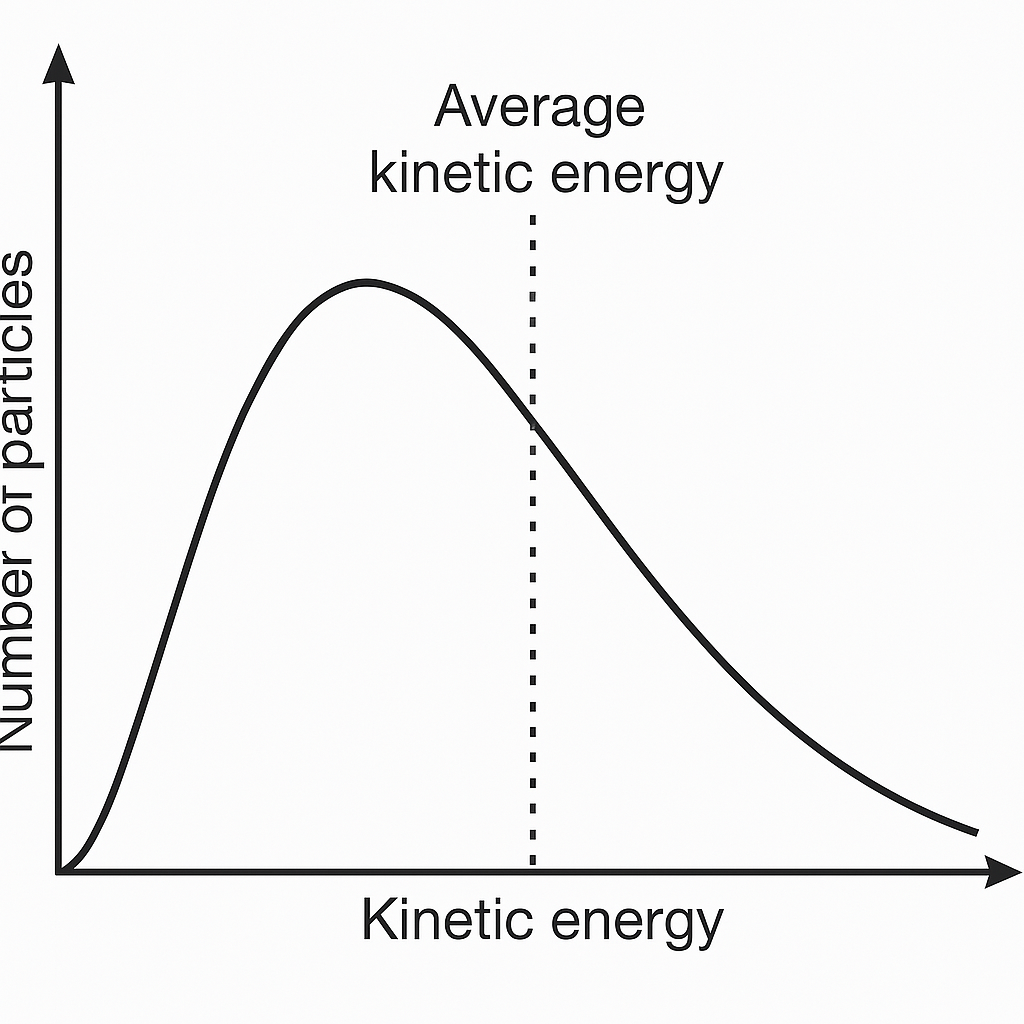
\includegraphics[width=\linewidth]{kinetic_energy.png} % Replace with actual image path if available
\caption{A typical distribution of kinetic energies among particles in a substance at a given temperature. Higher temperatures shift the average energy to the right and broaden the distribution.}
\label{fig:particle_distribution}
\end{marginfigure}

It's important to distinguish between temperature and thermal energy. A large body of water (like a swimming pool) at a lower temperature can contain significantly more thermal energy than a small cup of water at a higher temperature because it has vastly more particles, even if their average kinetic energy is lower.

\begin{stopandthink}
Consider a litre of water at 80°C and 10 litres of water at 20°C. Which has the higher temperature? Which contains more thermal energy? Explain your reasoning based on the particle model.
\end{stopandthink}

\marginpar{\textbf{\challengeicon\ Challenge:} Research the difference between translational, rotational, and vibrational kinetic energy for molecules. How do these contribute differently to the thermal energy of solids, liquids, and gases?}
\marginpar{\textbf{History:} The connection between heat and particle motion was solidified by scientists like James Prescott Joule in the mid-19th century, challenging the earlier 'caloric' theory of heat as a fluid.}
\marginnote{Related HSC Question: HSC2020Q14b}

\FloatBarrier

\section{Thermal Equilibrium}
\label{sec:thermal_equilibrium}
\FloatBarrier

When objects at different temperatures are brought into thermal contact, energy naturally flows from the hotter object to the colder one. This process continues until the objects reach a state of \textbf{thermal equilibrium}.
\marginnote{\textbf{thermal equilibrium}: State when objects in contact have no net heat flow between them.}

\begin{keyconcept}{Thermal Equilibrium}
Thermal equilibrium is the state reached when two or more objects in thermal contact cease to have any net transfer of thermal energy between them. At equilibrium, they are at the same temperature. This concept is fundamental to the \textbf{Zeroth Law of Thermodynamics}, which states that if two systems are each in thermal equilibrium with a third system, then they are in thermal equilibrium with each other.
\end{keyconcept}
\marginnote{\textbf{Zeroth Law of Thermodynamics}: If two systems are in thermal equilibrium with a third system, they are in thermal equilibrium with each other.}

\marginnote{Syllabus Ref: PH11-10 (ACSPH022)}
\marginnote{Bloom's Level: Analyse}
\marginnote{Literacy Skills: Define thermal equilibrium, Explain energy transfer directions, Summarise Zeroth Law.}
\marginnote{Numeracy Skills: Interpret equilibrium diagrams.}
\marginnote{Demo Video: See \href{https://youtu.be/gzy4YFuKg9A?si=0iKVL83P-tgttZ-Z}{this video} for a demonstration.}
\marginnote{Related HSC Question: HSC2019Q12a}

\begin{marginfigure}[0pt]
% Placeholder for thermal equilibrium diagram
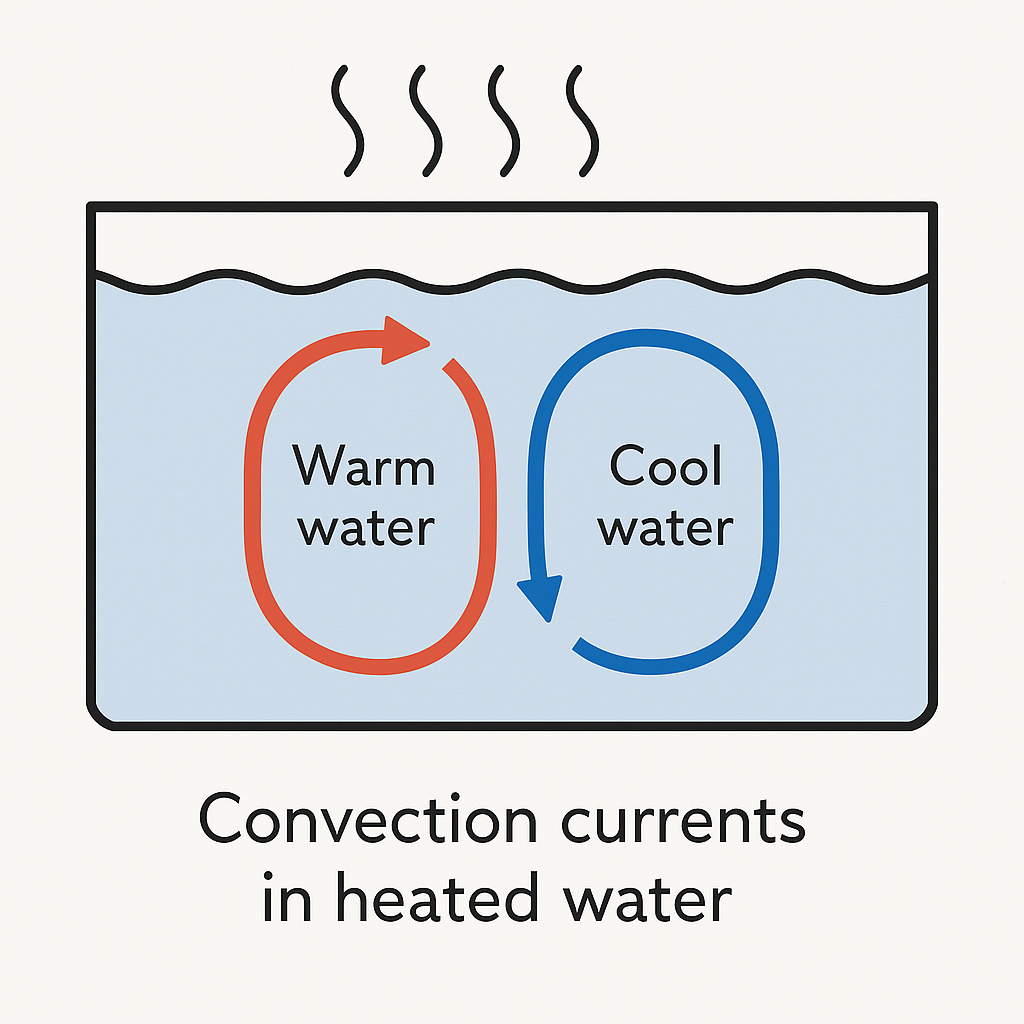
\includegraphics[width=\linewidth]{convection_currents.png} % Replace with actual image path if available
\caption{Two objects, A (hot) and B (cold), in thermal contact. Heat flows from A to B until T\(_A\) = T\(_B\), reaching thermal equilibrium. No net heat flow occurs at equilibrium.}
\label{fig:thermal_equilibrium}
\end{marginfigure}

Think about placing a thermometer in warm water. The thermometer's reading increases as thermal energy flows from the water to the thermometer. The reading stabilises when the thermometer reaches thermal equilibrium with the water – they are at the same temperature, and there is no further net energy transfer. Similarly, a hot drink left on a table will cool down until it reaches thermal equilibrium with the surrounding air.

\begin{stopandthink}
Why is the term 'net' transfer important when discussing thermal equilibrium? Do particles stop exchanging energy altogether?
\end{stopandthink}

\marginpar{\textbf{\challengeicon\ Challenge:} Consider three objects A, B, and C. If A and B are in thermal equilibrium, and B and C are in thermal equilibrium, what can you conclude about A and C? Explain how this relates to the function of a thermometer.}

\FloatBarrier

\section{Quantifying Heat Transfer: Specific Heat Capacity}
\label{sec:specific_heat}
\FloatBarrier

Different substances require different amounts of thermal energy to change their temperature by the same amount. This property is quantified by the \textbf{specific heat capacity}.
\marginnote{\textbf{specific heat capacity}: Energy needed to raise temperature of 1kg of material by 1K.}

\begin{keyconcept}{Specific Heat Capacity (c)}
Specific heat capacity (\(c\)) is the amount of thermal energy required to raise the temperature of one kilogram of a substance by one Kelvin (or one degree Celsius). Its unit is Joules per kilogram per Kelvin (J kg\(^{-1}\) K\(^{-1}\)) or Joules per kilogram per degree Celsius (J kg\(^{-1}\) °C\(^{-1}\)). The relationship between thermal energy transferred (\(Q\)), mass (\(m\)), specific heat capacity (\(c\)), and temperature change (\(\Delta T\)) is given by:
\begin{equation}
Q = mc\Delta T
\label{eq:specific_heat}
\end{equation}
where \(\Delta T = T_{final} - T_{initial}\). A positive \(Q\) indicates energy absorbed by the substance, while a negative \(Q\) indicates energy released.
\end{keyconcept}

\marginnote{Syllabus Ref: PH11-10 (ACSPH020)}
\marginnote{Working Scientifically: Problem Solving}
\marginnote{Bloom's Level: Apply}
\marginnote{Literacy Skills: Define specific heat capacity, Interpret heat capacity tables.}
\marginnote{Numeracy Skills: Calculate thermal energy and temperature change using Q=mc\textDelta T, Analyse experimental data.}
\marginnote{Video Resource: See \href{https://youtu.be/iTqmFteomjU?si=Of9TgyKBo4Yit2aI}{this video} for a visual explanation.}
\marginnote{Related HSC Question: HSC2021Q15}

\marginpar{\textbf{Math Link:} Ensure you can rearrange Equation \ref{eq:specific_heat} to solve for \(m\), \(c\), or \(\Delta T\). Pay close attention to units. A temperature *change* (\(\Delta T\)) is the same in Kelvin and Celsius, but the absolute temperatures are different.}

\begin{marginfigure}[-10pt]
\centering
\small % Smaller font for table
\begin{tabular}{lr}
\toprule
Substance & \(c\) (J kg\(^{-1}\) K\(^{-1}\)) \\
\midrule
Water (liquid) & 4186 \\
Ice (\(0^\circ\)C) & 2090 \\
Aluminium & 900 \\
Copper & 385 \\
Air (typical) & 1005 \\
\bottomrule
\end{tabular}
\caption{Approximate specific heat capacities of common substances. Note water's high value.}
\label{tab:specific_heat}
\end{marginfigure}

Water has a very high specific heat capacity compared to many other substances. This means it takes a lot of energy to heat water up, and water releases a lot of energy when it cools down. This property is crucial for climate regulation (large bodies of water moderate temperature changes) and in biological systems.

\begin{example}
How much thermal energy is required to heat 2.0 kg of water from 20°C to 80°C? (Use \(c_{water} = 4186\) J kg\(^{-1}\) K\(^{-1}\))

\textbf{Solution:}
Identify the known values:
\(m = 2.0\) kg
\(c = 4186\) J kg\(^{-1}\) K\(^{-1}\)
\(T_{initial} = 20\)°C
\(T_{final} = 80\)°C
Calculate the temperature change:
\(\Delta T = T_{final} - T_{initial} = 80°C - 20°C = 60\)°C (or 60 K)
Apply the formula:
\(Q = mc\Delta T\)
\(Q = (2.0\,\text{kg}) \times (4186\,\text{J kg}^{-1}\,\text{K}^{-1}) \times (60\,\text{K})\)
\(Q = 502320\) J
\(Q \approx 5.0 \times 10^5\) J (or 500 kJ)

Therefore, approximately 500 kJ of thermal energy is required.
\end{example}

\begin{investigation}{Determining Specific Heat Capacity Experimentally}
\textbf{Aim:} To experimentally determine the specific heat capacity of a metal block (e.g., aluminium).

\textbf{Apparatus:} Metal block of known mass, immersion heater, power supply, voltmeter, ammeter, thermometer, stopwatch, insulation.

\textbf{Method Outline:}
\begin{enumerate}
    \item Measure the mass (\(m\)) of the metal block.
    \item Record the initial temperature (\(T_{initial}\)) of the block.
    \item Insert the heater and thermometer into holes in the block. Ensure good thermal contact (a drop of oil can help). Insulate the block.
    \item Connect the heater to the power supply via the ammeter (series) and voltmeter (parallel).
    \item Start the stopwatch and switch on the power supply simultaneously. Record voltage (\(V\)) and current (\(I\)).
    \item Record the temperature (\(T\)) at regular intervals (e.g., every minute) for a set time (e.g., 10 minutes).
    \item Switch off the power supply. Record the maximum temperature reached (\(T_{final}\)).
\end{enumerate}

\textbf{Analysis:}
\begin{itemize}
    \item Calculate the electrical energy supplied: \(E = V \times I \times t\), where \(t\) is the total time in seconds.
    \item Assuming all electrical energy is converted to thermal energy absorbed by the block (\(Q \approx E\)), calculate \(\Delta T = T_{final} - T_{initial}\).
    \item Rearrange \(Q = mc\Delta T\) to find \(c\): \(c = \frac{Q}{m\Delta T} \approx \frac{VIt}{m\Delta T}\).
    \item Compare the experimental value with the known value and discuss sources of error (e.g., heat loss to surroundings, thermometer calibration, energy absorbed by heater/insulation).
\end{itemize}

\textbf{Safety Checklist:} [\ ] Ensure electrical connections are secure. [\ ] Do not touch the heater when hot. [\ ] Place apparatus away from edge of bench.

\textbf{Working Scientifically Focus:} Conducting Investigations (PH11/12-3), Processing Data (PH11/12-4), Problem Solving (PH11/12-6).
\end{investigation}

\marginpar{\textbf{\challengeicon\ Challenge:} How would you modify the specific heat capacity experiment to account for heat loss to the surroundings more accurately? Research techniques like the method of mixtures or continuous flow calorimetry.}

\FloatBarrier

\section{Mechanisms of Heat Transfer}
\label{sec:heat_transfer_mechanisms}
\FloatBarrier

Thermal energy transfer occurs through three primary mechanisms: conduction, convection, and radiation. Often, more than one mechanism is active simultaneously.

\marginnote{Syllabus Ref: PH11-10 (ACSPH016)}
\marginnote{Bloom's Level: Understand}
\marginnote{Literacy Skills: Describe energy transfer mechanisms, Compare mechanisms.}
\marginnote{Numeracy Skills: Interpret insulation performance graphs.}
\marginnote{Diagram Resource: See `heat-flow-hot-cold-objects.png`.}
\marginnote{Related HSC Question: HSC2018Q9a}

\subsection{Conduction}
\FloatBarrier % Add FloatBarrier before subsection content

\textbf{Conduction} is the transfer of thermal energy through direct contact and collisions between adjacent particles (atoms, molecules, electrons) without the bulk movement of the substance itself. It is the primary mechanism of heat transfer in solids.
\marginnote{\textbf{Conduction}: Heat transfer through direct contact between particles.}
\begin{itemize}
    \item **Mechanism:** Vibrating particles collide with neighbours, transferring kinetic energy. In metals, free electrons also play a significant role, making metals good thermal conductors.
    \item **Examples:** A metal spoon heating up in hot soup, heat travelling along an iron bar held in a flame.
    \item **Factors:** Depends on the material (thermal conductivity), temperature difference, cross-sectional area, and length.
\end{itemize}

\begin{marginfigure}[0pt]
% Placeholder for conduction diagram
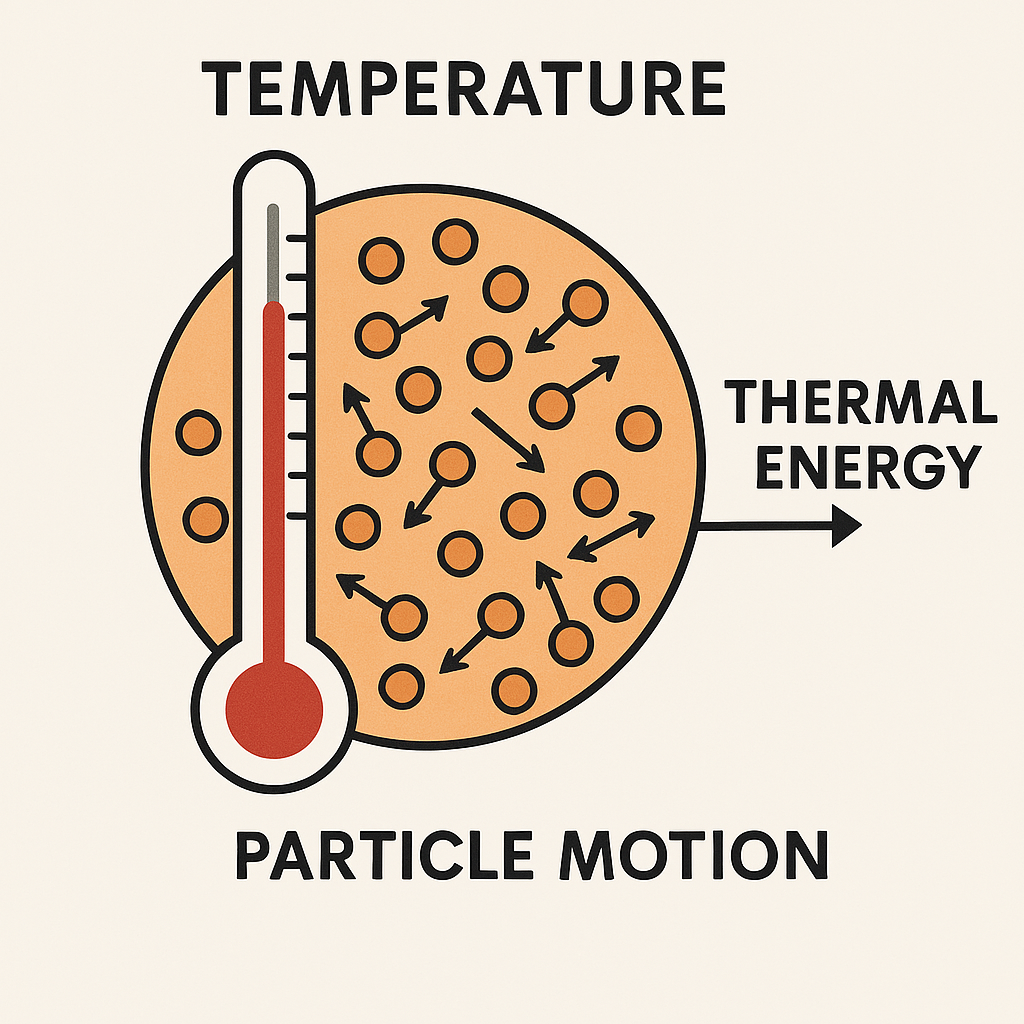
\includegraphics[width=\linewidth]{thermal_energy.png} % Replace with actual image path if available
\caption{Conduction: Heat energy transferred through particle collisions along a solid rod.}
\label{fig:conduction}
\end{marginfigure}

\subsection{Convection}
\FloatBarrier

\textbf{Convection} is the transfer of thermal energy through the bulk movement of fluids (liquids or gases). It occurs due to changes in density caused by temperature differences.
\marginnote{\textbf{Convection}: Heat transfer through the movement of fluids.}
\begin{itemize}
    \item **Mechanism:** When a fluid is heated from below, it expands, becomes less dense, and rises. Cooler, denser fluid sinks to take its place, creating a \textbf{convection current}.
    \item **Examples:** Boiling water in a pot, sea breezes, atmospheric circulation, central heating systems.
    \item **Types:** Natural convection (driven by density differences) and forced convection (driven by external means like fans or pumps).
\end{itemize}
\marginpar{\textbf{convection current}: Circular flow of fluid due to temperature-driven density differences.}

\begin{marginfigure}[-10pt]
% Placeholder for convection current diagram
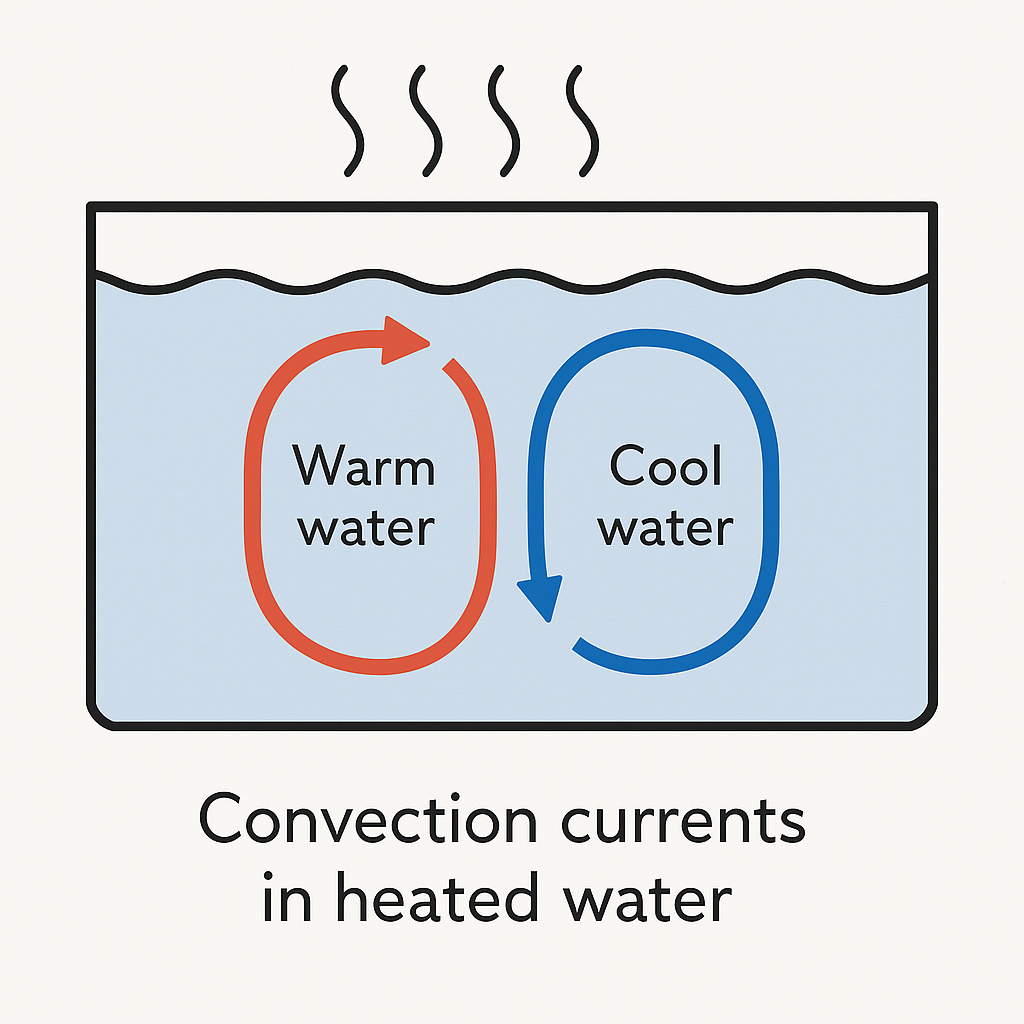
\includegraphics[width=\linewidth]{convection_currents.png} % Replace with actual image path if available
\caption{Convection currents in heated water. Warm, less dense water rises; cool, denser water sinks.}
\label{fig:convection}
\end{marginfigure}

\subsection{Radiation}
\FloatBarrier

\textbf{Radiation} is the transfer of thermal energy via electromagnetic waves (primarily infrared radiation). Unlike conduction and convection, radiation does not require a medium and can travel through a vacuum.
\marginnote{\textbf{Radiation}: Heat transfer via electromagnetic waves without requiring a medium.}
\begin{itemize}
    \item **Mechanism:** All objects above absolute zero emit thermal radiation. The rate of emission depends on temperature, surface area, and emissivity (a measure of how effectively a surface radiates). Hotter objects radiate more energy.
    \item **Examples:** Heat from the Sun reaching Earth, warmth felt near a campfire or radiator, thermal imaging cameras.
    \item **Surface Properties:** Dull, black surfaces are good absorbers and emitters of radiation, while shiny, light-coloured surfaces are poor absorbers/emitters but good reflectors.
\end{itemize}

\begin{marginfigure}[0pt]
% Placeholder for radiation diagram
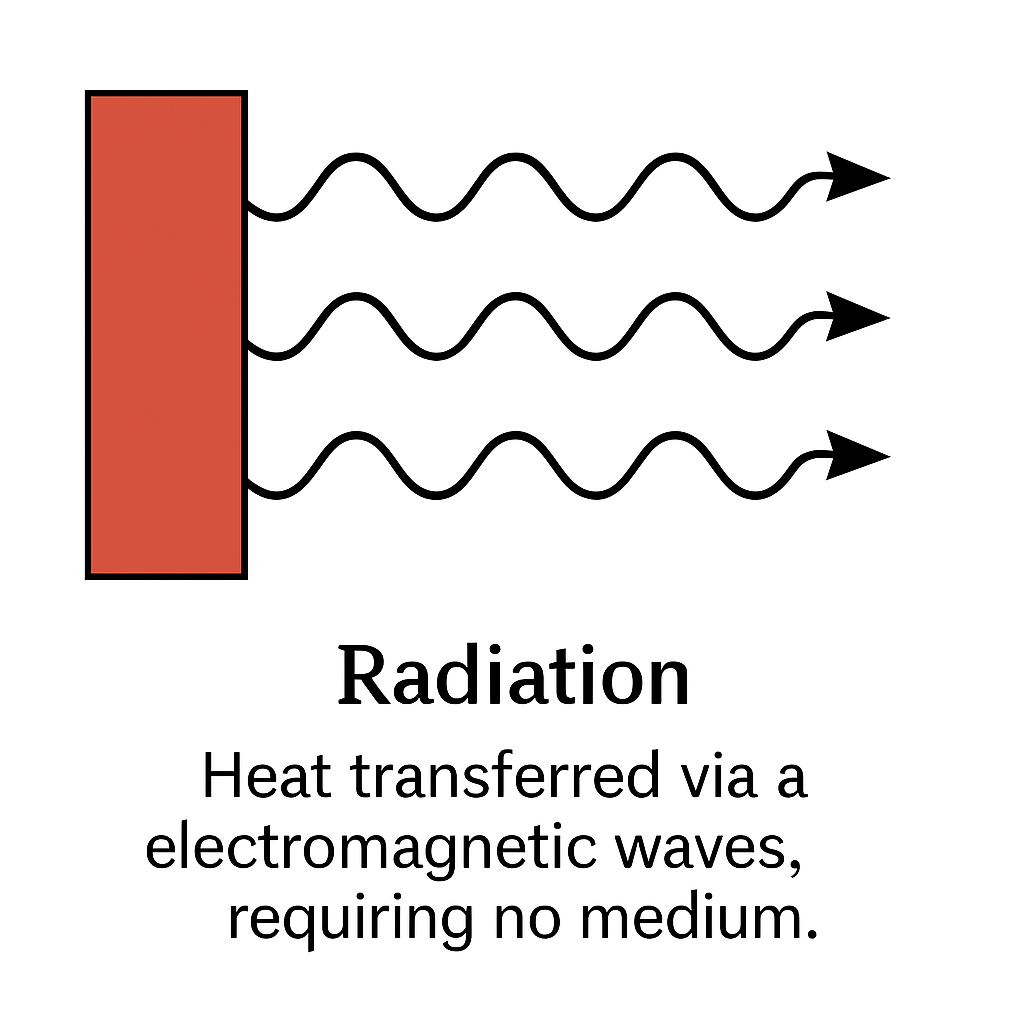
\includegraphics[width=\linewidth]{radiation.png} % Replace with actual image path if available
\caption{Radiation: Heat transferred via electromagnetic waves, requiring no medium.}
\label{fig:radiation}
\end{marginfigure}

\begin{stopandthink}
Explain how a thermos flask (vacuum flask) minimizes heat transfer by all three mechanisms (conduction, convection, radiation) to keep liquids hot or cold.
\end{stopandthink}

\marginpar{\textbf{\challengeicon\ Challenge:} Research the concept of thermal conductivity (for conduction), convective heat transfer coefficient (for convection), and emissivity (for radiation). How are these quantified and used in engineering applications like building insulation or heat exchanger design?}

\marginpar{\textbf{History:} Early theories struggled to explain heat transfer through vacuum until James Clerk Maxwell's theory of electromagnetism (1860s) provided the basis for understanding thermal radiation.}

\FloatBarrier

\section{Phase Changes and Latent Heat}
\label{sec:latent_heat}
\FloatBarrier

When a substance absorbs or releases thermal energy, its temperature may change (as described by specific heat capacity), or it may undergo a \textbf{phase change} (e.g., melting, boiling, freezing, condensing) at a constant temperature. The energy involved in phase changes is called \textbf{latent heat}.
\marginnote{\textbf{phase change}: Transformation between states of matter.}
\marginnote{\textbf{latent heat}: Energy required for phase change at constant temperature.}

\begin{keyconcept}{Latent Heat (L)}
Latent heat (\(L\)) is the thermal energy absorbed or released per unit mass of a substance during a phase change at constant temperature and pressure.
\begin{itemize}
    \item \textbf{Latent Heat of Fusion} (\(L_f\)): Energy required to change 1 kg of substance from solid to liquid (melting) or released when changing from liquid to solid (freezing).
    \item \textbf{Latent Heat of Vaporization} (\(L_v\)): Energy required to change 1 kg of substance from liquid to gas (boiling/evaporation) or released when changing from gas to liquid (condensation).
\end{itemize}
The thermal energy (\(Q\)) required for a mass (\(m\)) to undergo a phase change is given by:
\begin{equation}
Q = mL
\label{eq:latent_heat}
\end{equation}
The unit for latent heat is Joules per kilogram (J kg\(^{-1}\)).
\end{keyconcept}
\marginnote{\textbf{Latent Heat of Fusion}: Energy for solid-liquid transition.}
\marginnote{\textbf{Latent Heat of Vaporization}: Energy for liquid-gas transition.}

\marginnote{Syllabus Ref: PH11-10}
\marginnote{Working Scientifically: Processing Data and Information}
\marginnote{Bloom's Level: Analyse}
\marginnote{Literacy Skills: Interpret phase change graphs.}
\marginnote{Numeracy Skills: Calculate latent heat using Q=mL, Analyse heating/cooling curves rigorously.}
\marginnote{Video Resource: See \href{https://youtu.be/3itqmCtmJPc?si=kllbHNira3Vj8dnl}{this video} for a visual explanation.}
\marginnote{Related HSC Question: HSC2019Q13b}

\marginpar{\textbf{Math Link:} Be careful! Use \(Q=mc\Delta T\) when temperature changes, and \(Q=mL\) when phase changes occur at constant temperature. Problems often involve multiple steps combining both equations.}

\begin{marginfigure}[-20pt] % Adjust offset
% Placeholder for heating curve of water
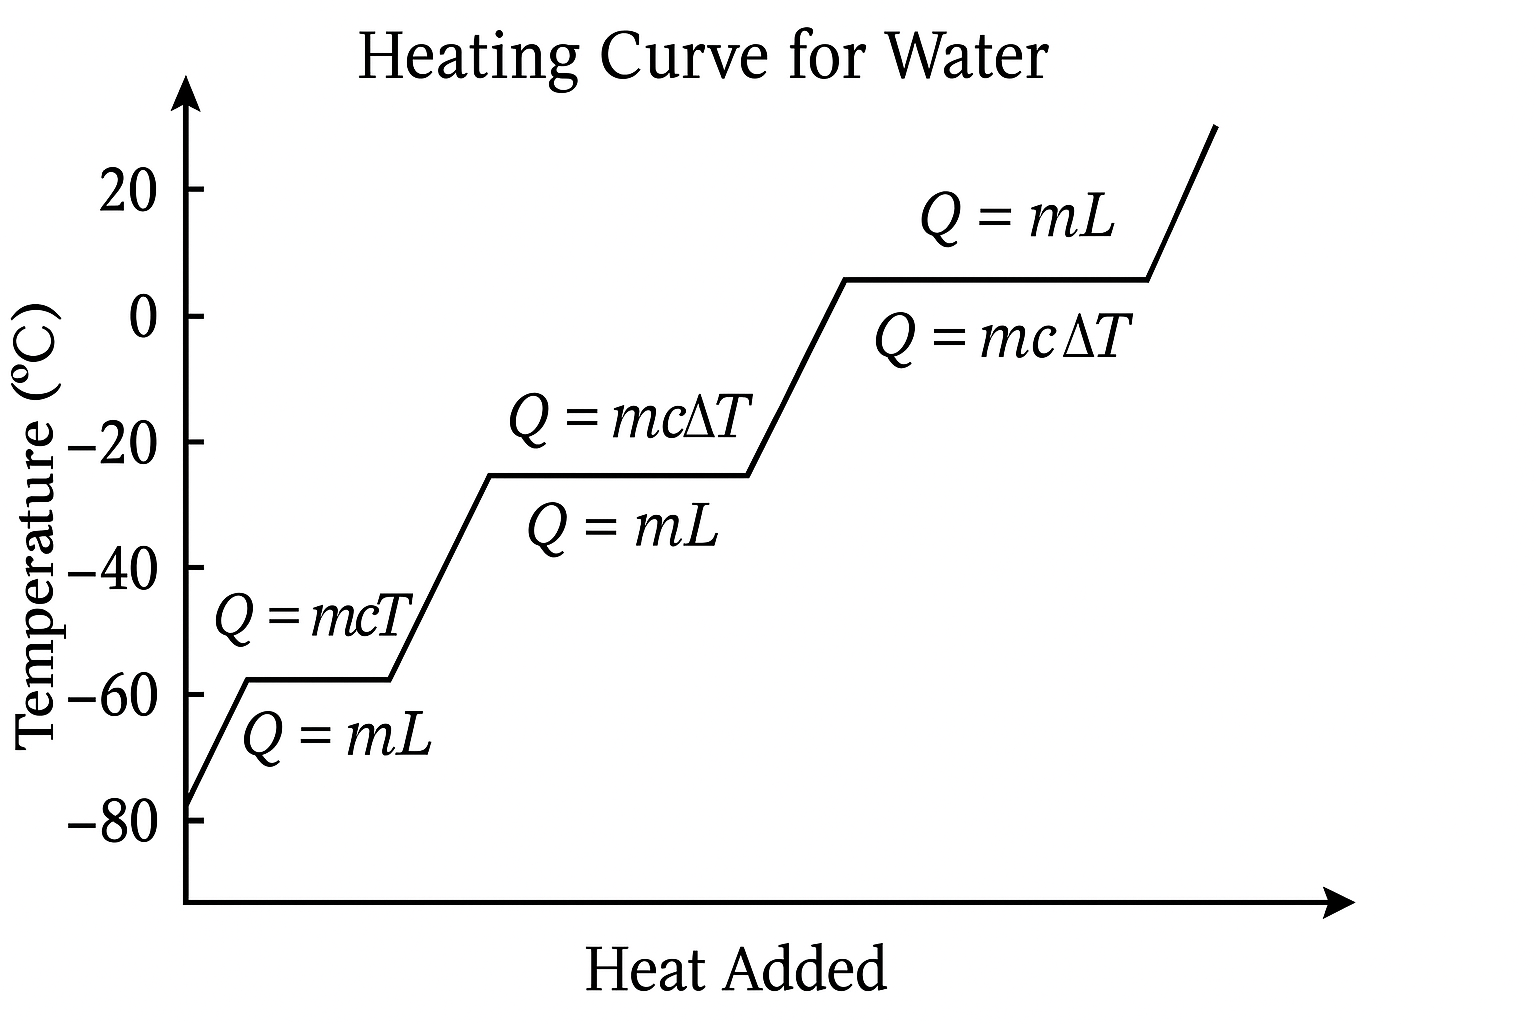
\includegraphics[width=\linewidth]{water_heating.png} % Replace with actual image path if available
\caption{Heating curve for water. Sloped sections represent temperature increases (Q=mc\textDelta T applies). Flat sections represent phase changes at constant temperature (Q=mL applies): melting at 0°C and boiling at 100°C.}
\label{fig:heating_curve}
\end{marginfigure}

During a phase change, the absorbed energy (latent heat) increases the potential energy of the particles (breaking intermolecular bonds) rather than their average kinetic energy (temperature). This is why the temperature remains constant during melting or boiling.

\begin{example}
Calculate the total thermal energy required to convert 500 g of ice at 0°C to steam at 100°C.
(Use \(L_f(\text{water}) = 3.34 \times 10^5\) J kg\(^{-1}\), \(c(\text{water}) = 4186\) J kg\(^{-1}\) K\(^{-1}\), \(L_v(\text{water}) = 2.26 \times 10^6\) J kg\(^{-1}\))

\textbf{Solution:}
This requires three steps:
1.  Melting the ice at 0°C: \(Q_1 = mL_f\)
2.  Heating the water from 0°C to 100°C: \(Q_2 = mc\Delta T\)
3.  Boiling the water at 100°C: \(Q_3 = mL_v\)

Convert mass to kg: \(m = 500\,\text{g} = 0.500\,\text{kg}\)
Calculate \(\Delta T\) for water heating: \(\Delta T = 100°C - 0°C = 100\) K

1.  \(Q_1 = (0.500\,\text{kg}) \times (3.34 \times 10^5\,\text{J kg}^{-1}) = 1.67 \times 10^5\) J
2.  \(Q_2 = (0.500\,\text{kg}) \times (4186\,\text{J kg}^{-1}\,\text{K}^{-1}) \times (100\,\text{K}) = 2.093 \times 10^5\) J
3.  \(Q_3 = (0.500\,\text{kg}) \times (2.26 \times 10^6\,\text{J kg}^{-1}) = 1.13 \times 10^6\) J

Total energy: \(Q_{total} = Q_1 + Q_2 + Q_3\)
\(Q_{total} = (1.67 + 2.093 + 11.3) \times 10^5\) J
\(Q_{total} = 15.063 \times 10^5\) J \(\approx 1.51 \times 10^6\) J (or 1.51 MJ)

Therefore, approximately 1.51 MJ of energy is required.
\end{example}

\begin{stopandthink}
Why does steam at 100°C cause more severe burns than water at 100°C? Relate your answer to latent heat.
\end{stopandthink}

\marginpar{\textbf{\challengeicon\ Challenge:} Investigate the phenomenon of evaporative cooling. Explain how the evaporation of sweat helps regulate body temperature, linking it to the latent heat of vaporization.}
\marginnote{Depth Study Idea: Experimentally determine the latent heat of fusion of ice using calorimetry. Identify key sources of uncertainty.}

\FloatBarrier

\section{Chapter Summary & Further Connections}
\label{sec:thermo_summary}
\FloatBarrier

This chapter explored fundamental thermodynamic concepts:
\begin{itemize}
    \item \textbf{Temperature} relates to the average kinetic energy of particles.
    \item \textbf{Thermal Energy} is the total internal energy.
    \item \textbf{Thermal Equilibrium} is reached when there is no net heat flow (equal temperatures).
    \item \textbf{Specific Heat Capacity} (\(Q = mc\Delta T\)) quantifies energy needed for temperature change.
    \item \textbf{Heat Transfer Mechanisms} are conduction, convection, and radiation.
    \item \textbf{Latent Heat} (\(Q = mL\)) quantifies energy needed for phase changes at constant temperature.
\end{itemize}

These principles have broad applications, from understanding weather patterns and climate change (linking to Environmental Science and the cross-curriculum priority of Sustainability) to designing efficient engines and refrigeration systems. The energy changes involved in phase transitions and chemical reactions (studied in Chemistry) are also governed by thermodynamic principles. Developing solutions to global energy challenges relies heavily on applying and advancing our understanding of thermodynamics.

\FloatBarrier

\section{Practice Questions}
\label{sec:thermo_questions}
\FloatBarrier

\begin{tieredquestions}{Basic}
\begin{enumerate}
    \item Define temperature in terms of particle motion.
    \item State the formula for calculating thermal energy change related to specific heat capacity, defining each term.
    \item List the three main mechanisms of heat transfer.
    \item What is latent heat? Give one example of where it is relevant.
    \item Calculate the energy required to heat 0.5 kg of aluminium from 20°C to 100°C. (Use \(c_{Al} = 900\) J kg\(^{-1}\) K\(^{-1}\))
\end{enumerate}
\end{tieredquestions}

\begin{tieredquestions}{Intermediate}
\begin{enumerate}
    \item Explain the difference between thermal energy and temperature using a macroscopic example (e.g., ocean vs boiling kettle).
    \item Describe the process of reaching thermal equilibrium between a hot metal block and cool water in a calorimeter.
    \item A 2.0 kW heater is used to heat 5.0 kg of water initially at 15°C for 3 minutes. Assuming no heat loss, calculate the final temperature of the water. (Use \(c_{water} = 4186\) J kg\(^{-1}\) K\(^{-1}\))
    \item Compare and contrast conduction and convection, giving examples where each is the dominant mode of heat transfer.
    \item Calculate the energy released when 200 g of steam at 100°C condenses to water at 100°C. (Use \(L_v(\text{water}) = 2.26 \times 10^6\) J kg\(^{-1}\))
    \item Sketch a cooling curve (Temperature vs Time) for a substance that starts as a gas, cools, condenses to a liquid, cools further, freezes to a solid, and finally cools as a solid. Label the sections corresponding to specific heat and latent heat.
\end{enumerate}
\end{tieredquestions}

\begin{tieredquestions}{Advanced}
\begin{enumerate}
    \item A 100 g copper block at 90°C is placed into 300 g of water at 20°C in an insulated container. Calculate the final equilibrium temperature, assuming no heat loss to the container. (Use \(c_{Cu} = 385\) J kg\(^{-1}\) K\(^{-1}\), \(c_{water} = 4186\) J kg\(^{-1}\) K\(^{-1}\)) \textit{Hint: Heat lost by copper = Heat gained by water.}
    \item Design an experiment to compare the effectiveness of different insulating materials (e.g., wool, foam, air gap) in reducing heat transfer by conduction and convection. Specify your independent, dependent, and controlled variables, and outline your method and data analysis approach. (Focus on experimental design and scientific process - PH11/12-3, PH11/12-6).
    \item (PISA-style) A company is designing a new type of solar water heater for residential use. They are considering two designs: one using copper pipes painted black, and another using plastic pipes with a selective coating that absorbs sunlight well but emits little infrared radiation. Analyse the potential advantages and disadvantages of each design in terms of heat absorption (radiation), heat transfer to the water (conduction/convection), and heat loss to the environment (all three mechanisms). Justify which design might be more efficient overall, considering different climate conditions. (Focus on applying concepts to a real-world problem, evaluating designs - PH11-10, PH11/12-6, PH11/12-7).
    \item Explain quantitatively why sweating is an effective cooling mechanism for the human body, even on a hot day when the surrounding air temperature might be higher than body temperature. Use the concept of latent heat of vaporization in your explanation.
    \item How much energy is required to convert 1.0 kg of ice initially at -10°C completely into steam at 110°C? You will need specific heat capacities for ice and steam, in addition to water, plus both latent heats. (Requires finding additional data - PH11/12-4). (Example values: \(c_{ice} \approx 2090\), \(c_{steam} \approx 2010\) J kg\(^{-1}\) K\(^{-1}\)).
\end{enumerate}
\end{tieredquestions}

\FloatBarrier % Final barrier for the chapter
